

\documentclass[11pt, a4paper]{article}
\renewcommand{\baselinestretch}{1.5}
\usepackage[utf8]{inputenc}
\usepackage{amsmath}
\usepackage{amsfonts}
\usepackage{mathtools}
\usepackage{bbm}
\usepackage{float}
\usepackage{array}
\usepackage{geometry}
\usepackage{amsfonts}
\usepackage{microtype}
\usepackage{accents}
\usepackage{relsize}
\usepackage{bm}
\usepackage{caption}
\usepackage{subcaption}
\usepackage{lscape}
\usepackage{pdflscape}
\geometry{
 a4paper,
 left=3cm,
 right=2cm,
 top=3cm,
 bottom=2cm
 }
\newcommand{\Lagr}{\mathcal{L}}
\usepackage{listings}
\usepackage[svgnames]{xcolor}
\lstset{language=R,
    basicstyle=\small\ttfamily,
    stringstyle=\color{DarkGreen},
    otherkeywords={0,1,2,3,4,5,6,7,8,9},
    morekeywords={TRUE,FALSE},
    deletekeywords={data,frame,length,as,character},
    keywordstyle=\color{blue},
    commentstyle=\color{DarkGreen},
}
\usepackage{amssymb}
\newcommand{\E}{\mathrm{E}}
\newcommand{\Var}{\mathrm{Var}}
\newcommand{\Cov}{\mathrm{Cov}}
\renewcommand{\P }{\mathrm{P }}
\renewcommand{\ln }{\mathrm{ln }}

\usepackage{natbib}
\bibliographystyle{chicago}






\begin{document}


\newgeometry{top=2.5cm}
\begingroup  
  \centering

   \small UNIVERSIDADE DE SÃO PAULO\\Faculdade de Economia, Administração e Contabilidade de Ribeirão Preto\\Programa de Pós-Graduação em Economia\\[10em]
     
  \Large Unemployment, Inflation and Violence: \\a VAR and cointegration approach for Brazil\\[10 em]
  
%  \Large CORRUPTION AND ECONOMIC GROWTH:\\ A CROSS-COUNTRY STUDY\\[5 em]

\begin{flushright}
\begin{minipage}[t]{0.5\textwidth}
\small Este trabalho foi apresentado na disciplina de Econometria III ministrada por Márcio P. Laurini e Sérgio Kannebley Júnior no segundo semestre de 2018. Programa de pós-graduação em economia da FEA RP USP.\\[5em]\par
\end{minipage}
\end{flushright}

\small Aluno: William Yasuhiko Nagai Suzuki \\ NºUSP: 8012391	\\   [5em]\par


%\begin{flushleft}
%    \textit{\small JEL classification:} K42; O43; O57 
%\end{flushleft}


\vfill{\small Ribeirão Preto\\ 2019}\\[5em]

\thispagestyle{empty}

\endgroup


\clearpage\mbox{}\thispagestyle{empty}\clearpage

\begin{abstract}


The objective of this work is to examine the relationship between unemployment, inflation and violence in Brazil using a vector autoregressive and vector error correction  models. Our hypothesis is that unemployment and inflation increase violence measures. We find evidence that unemployment and inflation have negative impact on many violence measures. We find that there is long-run relationship between the variables. The violence measures tested here are:  rape, homicides, vehicle theft, vehicle robbery, personal injury and death and felony murder. 

\end{abstract}



\section{Introduction}

There is great concern among economists and the government about the dynamics of unemployment and inflation and its impact on the well-being of the population. But what is the impact of worsening unemployment and inflation in measures closer to the common people's lives, like violence?
The objective of this work is to examine the relationship between unemployment, inflation and violence in Brazil using a vector autoregressive and vector error correction  models. Our hypothesis is that unemployment and inflation increase violence measures. 

\cite{becker1968} is the seminal paper that begun the investigation of the relationship between economic variables and crime. Becker's  argument is that when unemployment rises the marginal returns of legitimate earnings decrease. Thus creating  incentives to enter the criminal activity to people. 
In the literature there are arguments defending that unemployment have both positive and negative effects on crime: \cite{becker1968} argues that unemployment increases criminal motivations (motivational effect) and \cite{cantor_land_1985} argue that unemployment decrease criminal opportunities, because people start to buy less luxury goods and stay more at home, making it more difficult for it to be robbed for example (opportunity effect). 
Also the motivational effect of unemployment may be a long-run effect, because most people will consume their savings and use the welfare system first before entering the criminal activity, on the other hand the opportunity effect is felt more in the short-run \citep{tang2009}.


There is a difference between violent crime and property crime. The latter have an economic motivation and have been widely studied specially using cross-section and panel data \citep{saridakis2004}. But violent crime does not have necessarily an economic motivation and have greater space for research.

Increasing unemployment create incentives for people to enter the crime market, specially related to property crimes. Our hypothesis is that violent crimes increase due to social instability caused by unemployment. There is plenty of evidence showing that unemployment increase crime in general \citep{saridakis2011}. But it is not hard to see that families affected by poverty and lack of financial means to live suffer when unemployment and inflation increase. This is a channel for increasing violent crimes in the long-run. 

Our hypothesis is that inflation increase violent crimes through the rise of cost of living. If a family is going through economic hardship rising costs of living can increase the propensity of some to enter the illegal activity, and the social discontentment created by inflation can increase violent crimes.

\cite{saridakis2004} points that it is unlikely that unemployment may have an impact in violent crimes committed by the group of hardened criminals. But he also states that the persistence of unemployment induces people to enter the criminal activity and increase cases of violent crimes. The author studies the relationship between socio-economic variables and violence in the USA from 1960 to 2000.
Saridakis finds no long-run relationship between socio-economic variables and violence. But he finds short-run relationship. His violence variables include: murder, rape and assault. He find that unemployment play an unimportant role in explaining violence. 

\cite{tang2009} studies the relationship among crime, unemployment and inflation in Malaysia. He found a long-run equilibrium relationship between unemployment, inflation and crime. There is Granger causality from unemployment and inflation to crime, but there is no reverse causality. The cointegrating vector shows that increasing unemployment and inflation increase crime. He uses data from 1970 to 2006 with violent crimes and property crimes.


\cite{saridakis2011} using cointegration analyzes the long run relationthip between violent crimes, economic conditions, justice system and beer comsuption in England and Wales. He finds that there is long-run relationship between economic variables, police deterrence and aggravated assault. 

Using cointegration \cite{santos_kassouf2014} investigate how violent crime is related with unemployment and law-enforcement activities in the city of São Paulo. They find that violent crimes are positively related to unemployment and negatively related to real wages. In the same line
\cite{corman1987} use a VAR model to study the relatioship between unemployment, demographics and police activity and property-related felony crimes, for 1970 to 1984 in New York city. They find a weak positive relation between unemployment and violence.  

In this work we find that for most types of violent crimes there is relationship between unemployment and inflation and violent crime. \cite{santos_kassouf2014} do not find short-run relationship between those variables. The authors use data about homicide and robbery aggravated by death. 
In general the literature find that there is weak relationship between the three variables. 
Some papers find cointegration relationship between the variables and others find short-run relationship only, as in this work we find that not all variables are significant but they show the expected behavior: that unemployment and inflation increase violent crimes.










\section{Methodology}

\subsection{Vector Autoregression}

We apply vector autoregressive models for unemployment, inflation and violent crime. The next section will explain and analyze each of the violent crime measures. The VAR(p) model is:
$$ y_t = \mu + \Phi_1 y_{t-1} + \Phi_2 y_{t-2} + \dots + \Phi_p y_{t-p} + \varepsilon_t  $$
where $ \varepsilon_t $ is a vector of error stochastic process with $ \E[\varepsilon_t] = 0 $, $\Var[\varepsilon_t ] = \Omega$. $y_t$ is the vector containing unemployment ($u_t$), inflation ($\pi_t$) and a variable of violence ($v_t$). That is: $ y_t = (u_t,\pi_t, v_t )' $. The matrices $ \Phi_i$ for $i = 1, \dots, p$ are $3 \times 3$ and are the coefficient matrices. The VAR model can be estimated using ordinary least square in each of the equations. As our standard procedure we use the Schwartz criterion to determine the number of lags. 

After estimating the model we investigate the presence of Grange causality. We verify if $(u_t,\pi_t)$ Grange-cause $v_t$. We also test the other way around, some how $v_t$ Granger-causing $(u_t,\pi_t)$, which in theory does not make sense. 
The test of $(u_t,\pi_t)$ Grange-causing $v_t$ verifies if the coefficients of $u_t$ and $\pi_t$ in the VAR equation of $v_t$ are significant or not. 
Which means that Granger causality test verifies if a group of variables $(u_t,\pi_t)$ help to explain another group of variables $v_t$. Therefore Granger causality does not imply true causality or theory driven causality, in this case the theory agrees with Granger causality.

We apply impulse response analysis on the estimated VAR models. Following \cite{sims1980} we can estimate
$$ B y_t = c + \Gamma_1 y_{t-1} + \Gamma_2 y_{t-2} + \dots + \Gamma_p y_{t-p} + \eta_t $$
where 
$$ B = \begin{bmatrix}
1           & 0 & 0 \\
-\beta_{21} & 1 & 0    \\
-\beta_{31} & -\beta_{32} & 1   \\
\end{bmatrix} $$
note that  $y_t = (u_t,\pi_t, v_t )'$ with three variables. $\eta_t$ have a diagonal variance-covariance matrix. This specification implies that a hypothesis of causality between the innovation terms of each variable $u_t, \pi_t, v_t$. In this case the hypothesis is that 
$$ u_t \rightarrow \pi_t \rightarrow v_t $$
that is, unemployment's innovation is independent and it causes inflation's innovation and both of the former cause violence's innovation. 

Then the Wold's representation of the process is:
$$ y_t = \mu + \Theta_0 \eta_t + \Theta_1 \eta_{t-1} + \Theta_2 \eta_{t-2} + \dots  $$
$\eta_t$ are independent shocks, from which we can calculate the partial derivatives, for example the IRF of $v_t$ caused by shocks of $u_t$ in $s$ periods ahead of $t$:
$$ \frac{\partial v_{t+s} }{\partial \eta_{u,t}  } = \frac{\partial v_{t} }{\partial \eta_{u,t-s}} = \theta^{s}_{3,1}  $$
where $\theta^{s}_{3,1}$ is the coefficient of position $(3,1)$ of matrix $\Theta_s$, note that $v_t$ is in the third position and unemployment is in the first position of vector $y_t$. $\{\eta_{u,t}\}$ is the innovation process  of unemployment. 
The IRF graph of violence with unemployment shocks  is made from the the values $\theta^{s}_{3,1} $ for $s = 1, 2, 3, \dots$.

From the estimated VAR models we build the forecast error variance decomposition (FEVD). Our interest is in answering: what portion of the forecasting error of $v_{T+h}$ is caused by shocks in $\eta_j$, where $j \in \{u,\pi,v \}$. Where $T$ is the number of time periods available in the sample, and $h$ is the steps ahead.

For the violence variable specially we know that
$$ v_{T+h} - v_{T+h|T} = \sum\limits^{h-1}_{s=1} \theta^{s}_{3,1} \eta_{u,T+h-s} + \sum\limits^{h-1}_{s=1} \theta^{s}_{3,2} \eta_{\pi,T+h-s} + \sum\limits^{h-1}_{s=1} \theta^{s}_{3,3} \eta_{v,T+h-s} $$
taking the variance
$$ \Var[v_{T+h} - v_{T+h|T}] =  \sigma^2_{u} \sum\limits^{h-1}_{s=1} ( \theta^{s}_{3,1}  )^2 +  \sigma^2_{\pi} \sum\limits^{h-1}_{s=1} ( \theta^{s}_{3,2}  )^2 +  \sigma^2_{v} \sum\limits^{h-1}_{s=1} ( \theta^{s}_{3,3}  )^2 $$
where $\sigma^2_{j} := \Var[\eta_{j,t}]$ for all $t$ and $j \in \{u,\pi,v \}$.


\subsection{Cointegration}

Some of the variables are not stationary, hence we apply a cointegration test. The variables $u_t,\pi_t$ and $v_t$ are  cointegrated if exists $\beta = (1, -\beta_1, - \beta_2)'$ such that $ \beta' y_t = \varepsilon_t $  is stationary.  $\beta' y_t$ is called the long-run equilibrium relationship, the idea is that there are economic forces that draw the level of unemployment, inflation and violence together so that they cannot drift too much apart. \cite{tang2009} and \cite{saridakis2011} found long-run relationships in their studies, but \cite{santos_kassouf2014}
do not find cointegration relationship. All of those studies have some socio-economic and violent crime variable in their analysis.

We use the Johansen cointegration test to determine the number of cointegrating relations. After finding the cointegration vector(s) we apply the vector error correction model:
$$ \Delta y_t = c + \alpha \beta'y_t + \Psi_1 \Delta y_{t-1} + \dots + \Psi_{p-1} \Delta y_{t-p+1} + \eta_t $$
which is a restricted VAR, where $p$ is the number of lags of the underlying VAR model; the vector  $\alpha$ is $3 \times r$ is called the adjustment coefficients, they tell the speed with which the variables $\Delta u_t$, $\Delta \pi_t$ and $ \Delta v_t$ adjust to the long-run relationship, if some of the values in $\alpha$ are zero it tells that the variable does not adjust to the long-run relationship. For example, let $\alpha = (\alpha_u, \alpha_\pi, \alpha_v)'$ and let $\alpha_u = 0$ then we say that $u_t$ is weakly exogenous. $r$ is the number of cointegrating relations.

We apply a cointegration test on unemployment, inflation and violence we expect that specially the adjustment coefficient of violence be different from zero, because the other two variables are the economic background that determine social variables like crime. But the adjustment coefficients ($\alpha_u, \alpha_\pi$)  of unemployment and inflation can be different from zero because they can adjust to the long-run equilibrium relationship of each other in a Phillips curve. 



\section{Data}


The variable of unemployment is obtained through the site of the Brazilian Institute of Geography and Statistics (IBGE). The variable was built using the surveys of PNAD asking if the person was employed or looking for job in the last week. The frequency of the data is monthly.

Inflation data is the IPCA (Índice de Preços ao Consumidor Amplo) it captures the price levels of a bundle of goods, giving enphasis in metropolitan regions of Brazil, this is found in the site of IBGE. We apply the monthly rate of change of IPCA.

Violence variables are available in the site of Ministry of Justice of Brazil. The data have monthly information on the number of occurrences of violent crimes in each municipality. This is a dataset built  using reports of the civil police. There are other institutions of public security, for example, the  military police that have a strong presence in each state. So our data does not capture all cases of reported crimes, and many of the violent crimes are under reported.

In the \textbf{Results } section we will consider the violence variable $v_t$ as:
\begin{small}
\begin{itemize}
\item Rape
\item Homicides
\item Vehicle Theft
\item Vehicle Robbery
\item Personal Injury and Death
\item Felony Murder
\end{itemize}
\end{small}


All the referred violence variables are used in number of cases. The difference between vehicle theft and vehicle robbery is that theft does not involve the presence of the victim robbery is assault. Personal injury  and death occurs when the victim is injured but do not die on the spot, he dies some hours or days  later, hence the objective of the offender was not to kill. Felony murder is robbery followed by assassination. The word ``felony" usually is used to refer to grave crimes, and is used to differentiate it from petty crimes which are considered minor crimes.


Our time span is January 2004 to February 2016 there are 146 periods. Tables \ref{fig:1} and \ref{fig:2} show the time series for all variables used.


\begin{figure}[H]
\caption{}
\centering
%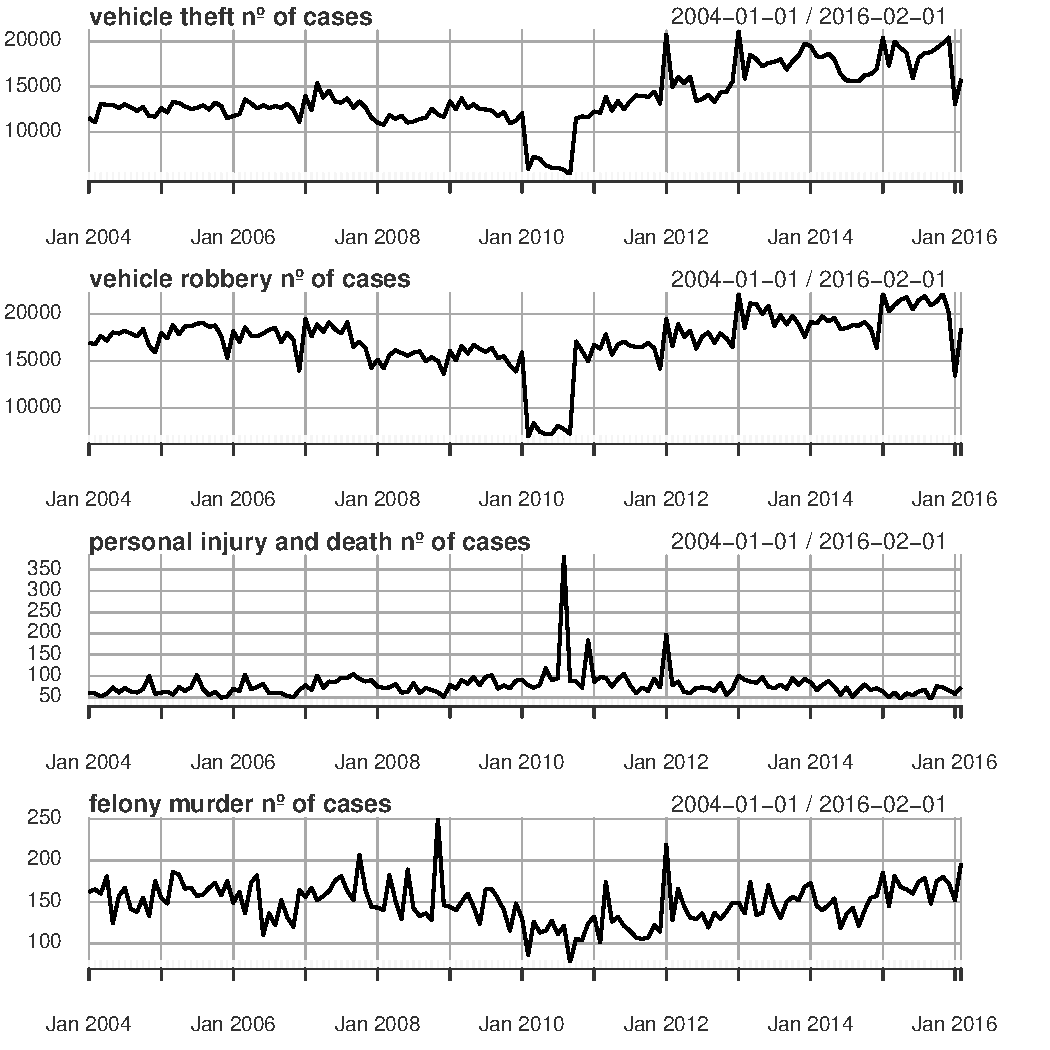
\includegraphics[width=\linewidth]{graph2}
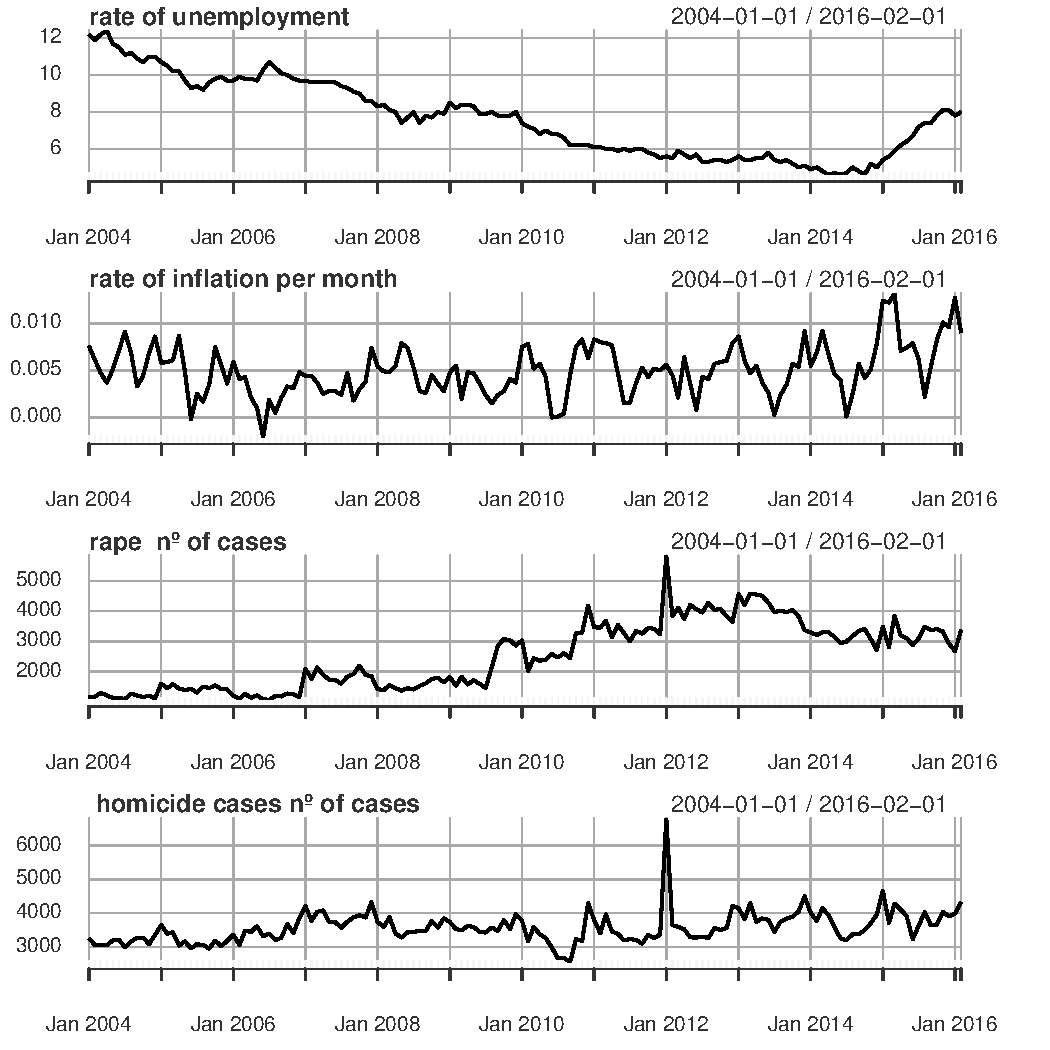
\includegraphics[width=15cm]{graph1}
\label{fig:1}
\end{figure}

\begin{figure}[H]
\caption{}
\centering
%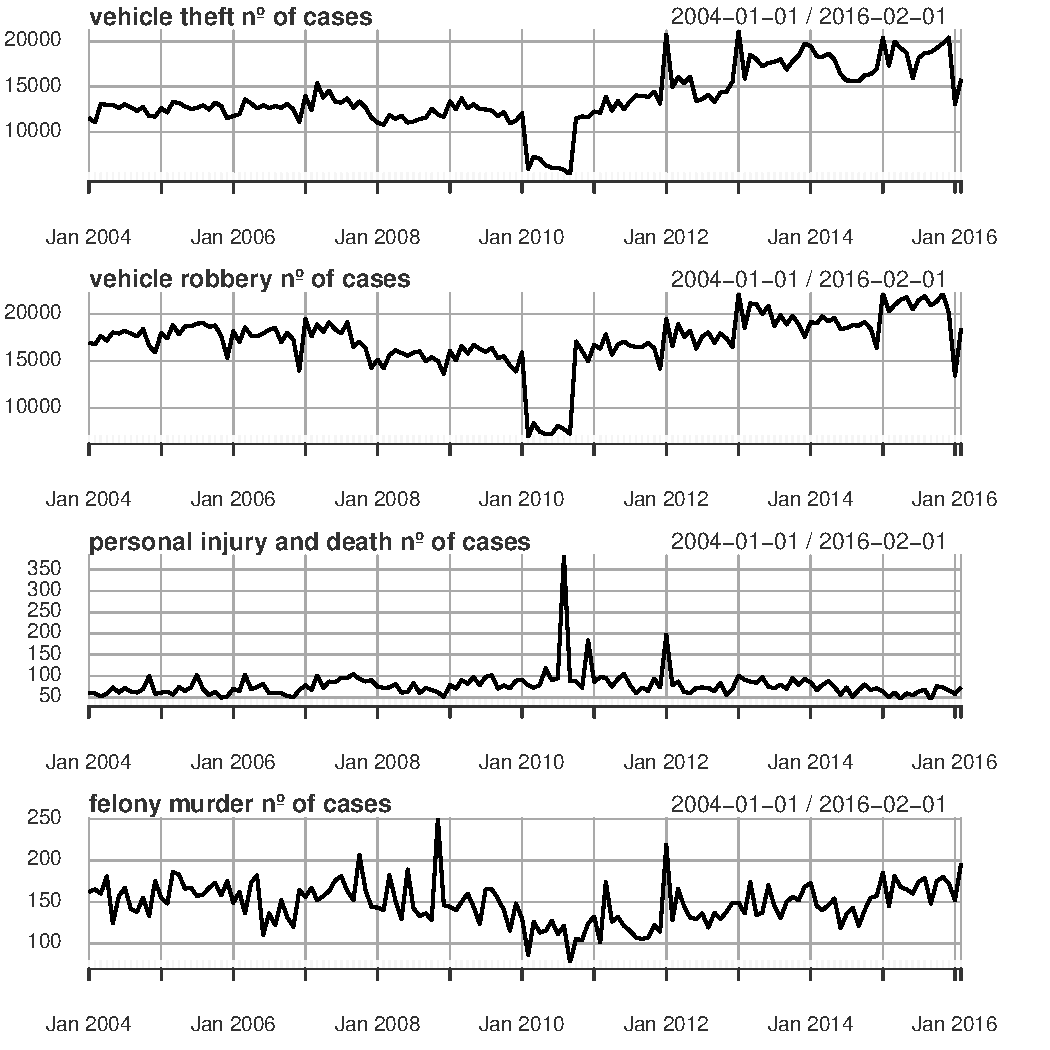
\includegraphics[width=\linewidth]{graph2}
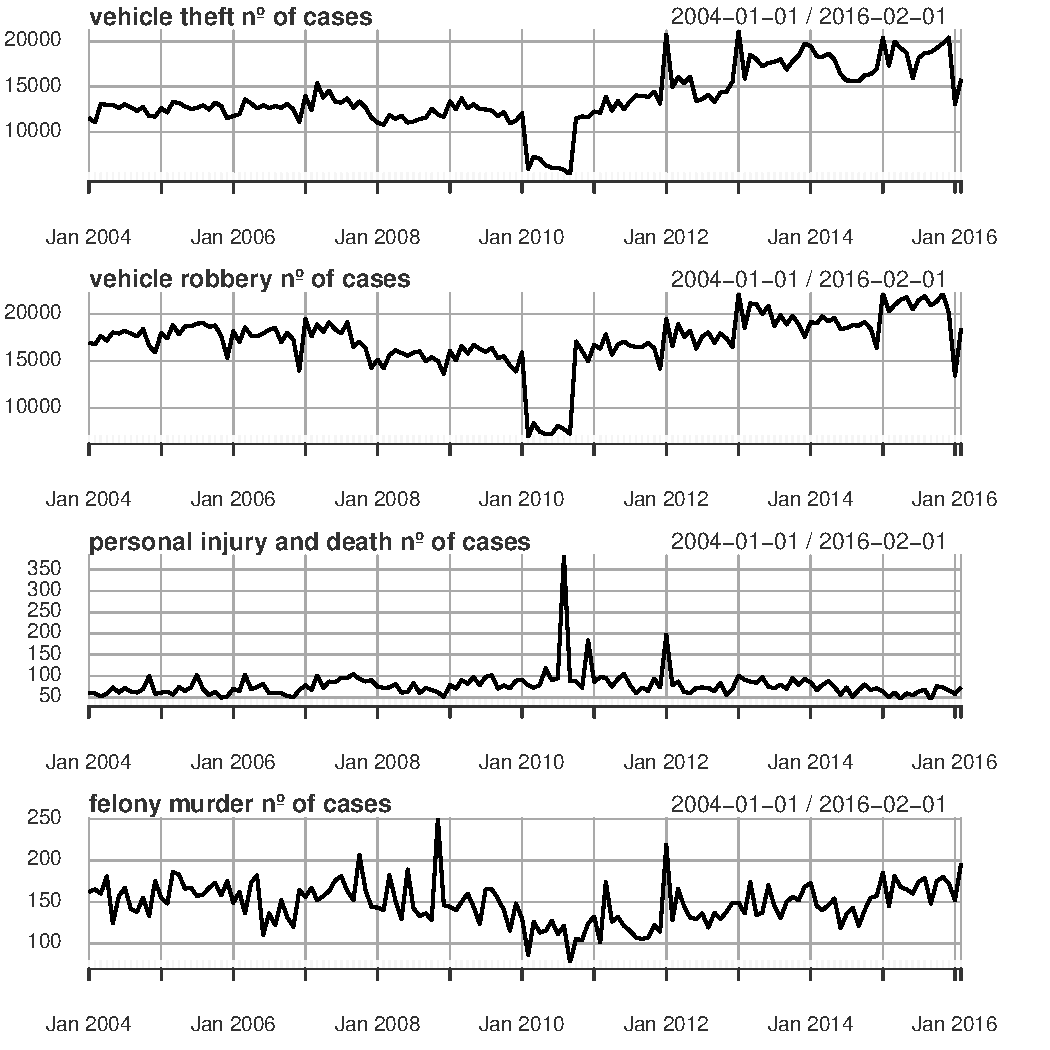
\includegraphics[width=15cm]{graph2}
\label{fig:2}
\end{figure}





\begin{table}[H]
\centering 
\caption{Augmented Dickey-Fuller tests}
\label{tab:adf.tests}
\begin{tabular}{l c c c}\hline\hline
\textbf{Variable} & \textbf{ADF}
 & \textbf{Type}& \textbf{Lags} \\ \hline

Unemployment & 0.379 & drift and trend  & 2 \\
Inflation & -5.23* & drift & 1 \\
Rape & -1.65 & drift and trend & 4 \\
Homicide & -7.38* & drift & 0 \\
Vehicle Theft & -3.41   & drift   &  0 \\
Vehicle Robbery & -4.18* & drift  &  0 \\
Personal Injury and Death & -10.30*  & drift   & 0  \\
Felony Murder & -8.52*   & drift    & 0   \\
\hline\hline
\multicolumn{4}{l}{\footnotesize *  $p \leq 0.01$}\\
\end{tabular}
\end{table}

Unemployment, rape and Vehicle theft are non-stationary. Inflation, homicide, vehicle robbery, personal injury and death and felony murder are all stationary. Felony murder can be non-stationary depending on the number of lags and type of deterministic terms, for example, with 4 lags and with drift and trend felony murder is non-stationary. This is important because further we apply a cointegration test on the variables: unemployment, inflation and felony murder.


\section{Results}

\subsection{VAR analysis}

Table \ref{tab:VAR_results1} below show the estimations of the VAR models with lags chosen by the Schwarz criterion. In all cases the chosen number of lags was 1. 
The equation of violence measure is the only one of interest, hence equations for unemployment and inflation are omitted. This is because our hypothesis is that the economic conditions are the ones that affect violence, not the other way around. 

We have six measures of violence and we apply with each a VAR model with $ y_t = (u_t,\pi_t, v_t )' $, where $u_t$ is the rate of unemployment per month, $\pi_t$ is the monthly rate of inflation and $v_t$ is one of the measures of violence. 
In Table \ref{tab:VAR_results1}, ``Normality" shows the results of the Jarque-Bera test on the residuals of the equation, for none of them we find residuals with Gaussian distribution. 
``Serial Cor." shows the result of Portmanteau test for serial correlation in the residuals. ``Granger  $ (u,\pi \rightarrow v  )$" shows the p-value of the Granger causality test for unemployment and inflation Granger causing violence. 

The variables of rape and vehicle theft are the ones that do not have significant estimates for unemployment or inflation, and those are the variables that do not show significant p-value in the Granger causality test.  Homicide, vehicle robbery, personal injury and death and felony murder show significant values for unemployment or inflation, hence they show significant values for Granger causality test. That is, for those variables are is indications that unemployment and/or inflation do Granger cause violence. All the estimates in Table \ref{tab:VAR_results1} are positive, that is what we expect: a positive shock in unemployment or inflation increase violence. The equation of homicide is the only one that showed no serial correlation. And felony murder is the only one that showed statistically significant impact of inflation.   




Graphs \ref{fig:graph_irf1} and \ref{fig:graph_irf2} show the impulse response functions of violence measures to shocks of unemployment and inflation. In figure \ref{fig:graph_irf2} we also have the IRF for VAR estimates with 3 lags, that is analyzed further. 
The IRF of  1 lagged models all show that a positive shock in unemployment increase violence, the impact have long-run consequences even after 20 months the shock continues to have effect. For homicide, note that there is a slight increase in the effect.
The $95\%$ confidence band of unemployment shocks is wider for the models that showed no significance for unemployment. For some variables there is no significant estimates of unemployment but they all show the same behavior, which means that although they are not statistically significant that does not mean that unemployment does not have impact on violence for those measurements, the issue is that they have too much variance.

For the inflation shocks, note that for almost all violence measures the impact increases till around 3 to 4 months and then slowly declines. This happens to all violence measures, although they may have different motivations, the same observation can be made for unemployment. Note that the inflation impact decreases but still takes a long time to return to zero. 








\begin{landscape}

\begin{table}[H]
\centering 
\caption{VAR results}
\label{tab:VAR_results1}
\begin{tabular}{l l l l l l l }\hline\hline 
   & \multicolumn{4  }{c   } {Explained Variables  } \\
Regressors & \textbf{Rape} & \textbf{Homicide} & \textbf{Vehicle }  & \textbf{Vehicle }  & \textbf{Personal Injury } & \textbf{Felony } \\ 
  & & &  \textbf{ Theft}  &   \textbf{ Robbery}       & \textbf{ and Death} & \textbf{Murder}  \\ \hline
$u_{t-1}$ & 5.824 & 39.56** & 60.43 & 10.99* & 4.347*** & 4.917*** \\
$\pi_{t-1}$ & 14170 & 23140  & 60240 &  90890 &  1579   & 3064***  \\
$v_{t-1}$ & 0.956*** & 0.878***  & 0.942*** &  0.9208*** & 0.438***    & 0.631***  \\
Normality  & no & no  & no & no  &  no  &  no   \\
Serial Cor. & yes & no  & yes & yes  & yes  &  yes    \\
Granger  $ (u,\pi \rightarrow v  )$ & 0.1965  & 0.02027    & 0.2054 & 0.08943 & 0 & 0  \\
\hline\hline
\multicolumn{4}{l}{\footnotesize *  $p < 0.10$, **  $p < 0.05$, ***  $p < 0.01$}\\
\end{tabular}
\end{table}


\end{landscape}








\begin{figure}[H]
\caption{IRF graphs}
\centering
%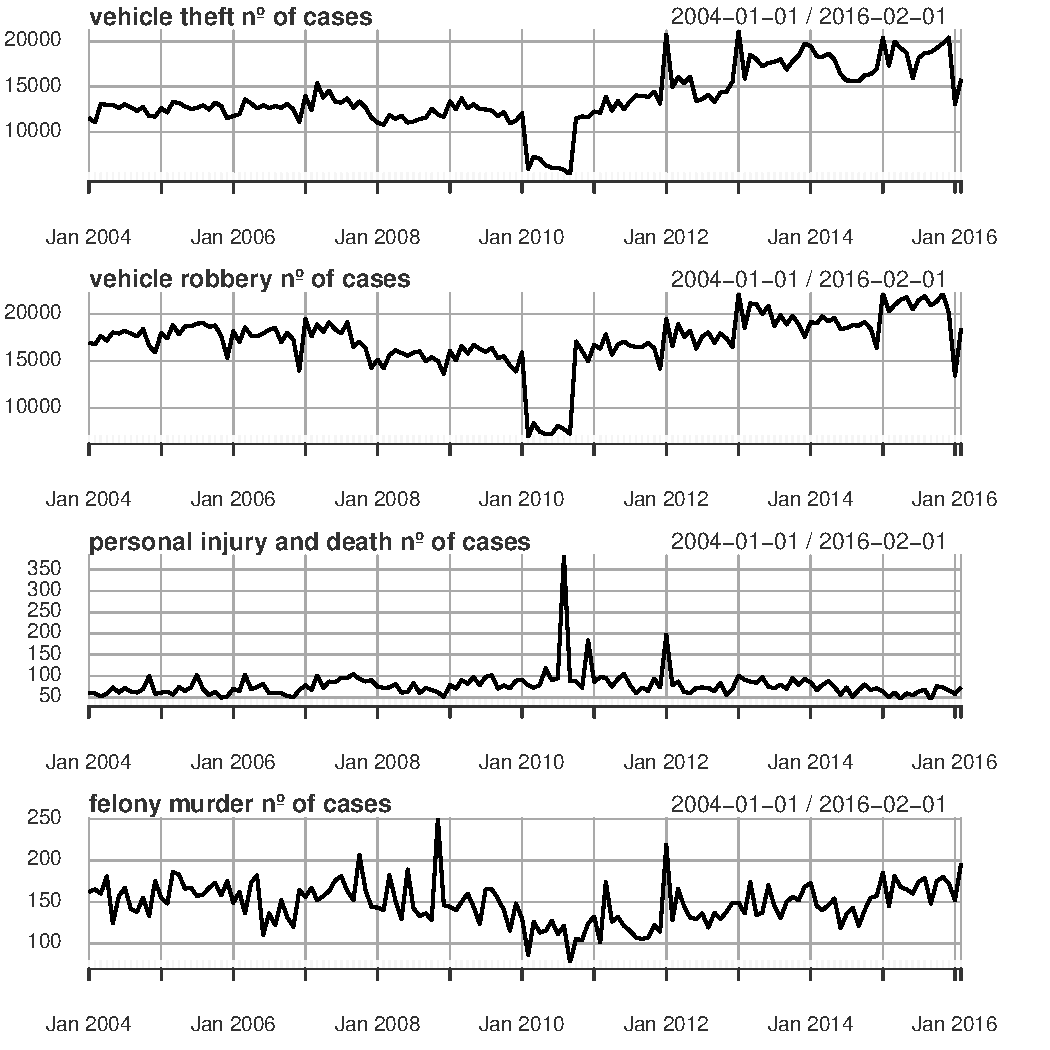
\includegraphics[width=\linewidth]{graph2}
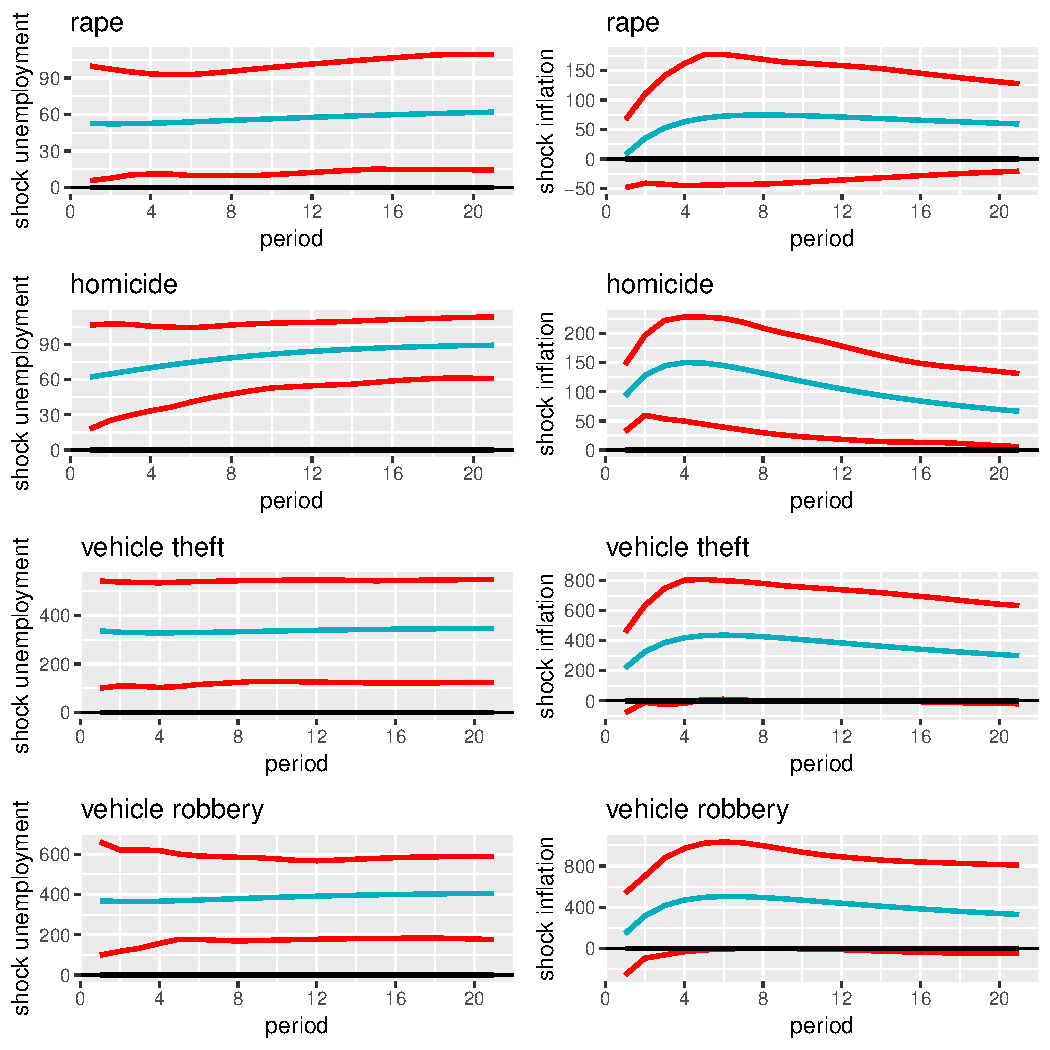
\includegraphics[width=15cm]{graph_irf1}
\label{fig:graph_irf1}
\end{figure}




\begin{figure}[H]
\caption{IRF graphs}
\centering
%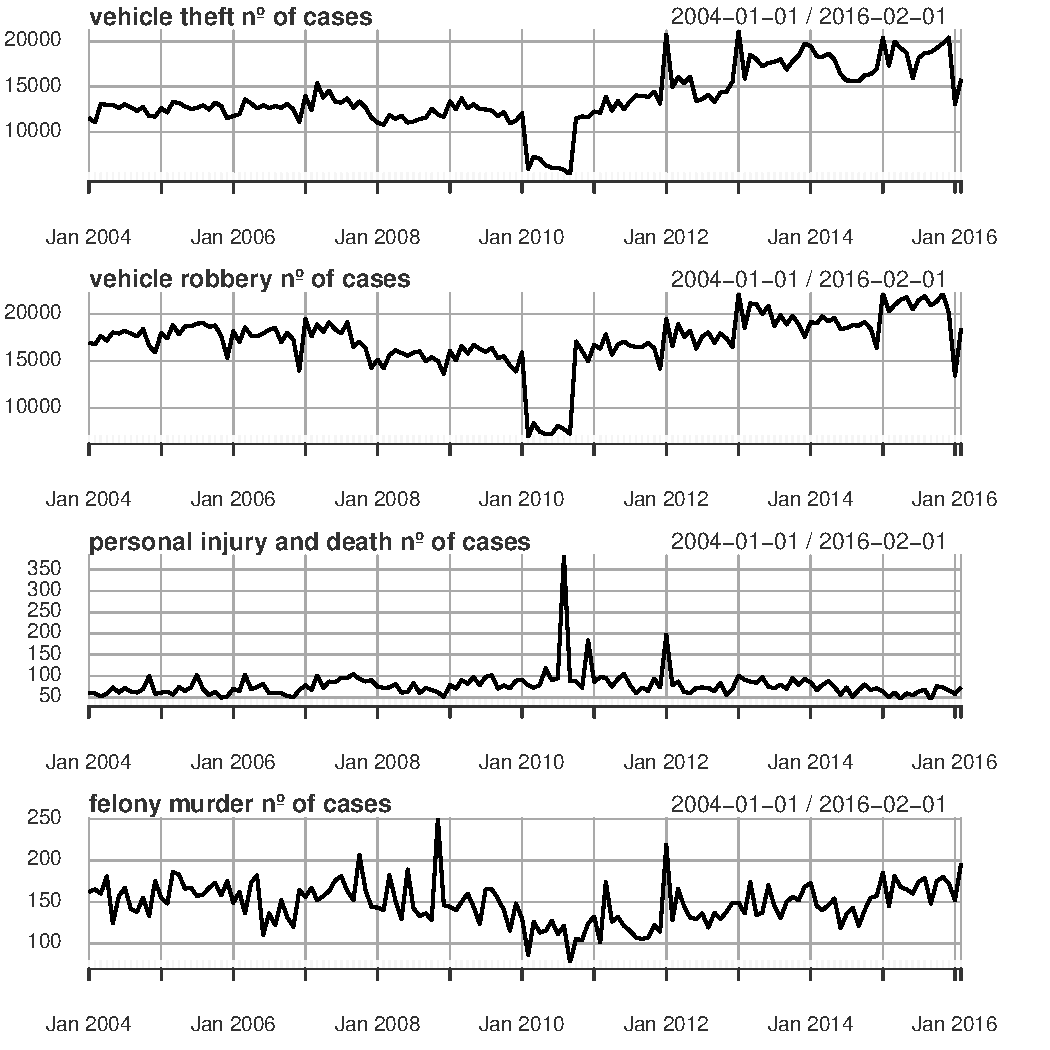
\includegraphics[width=\linewidth]{graph2}
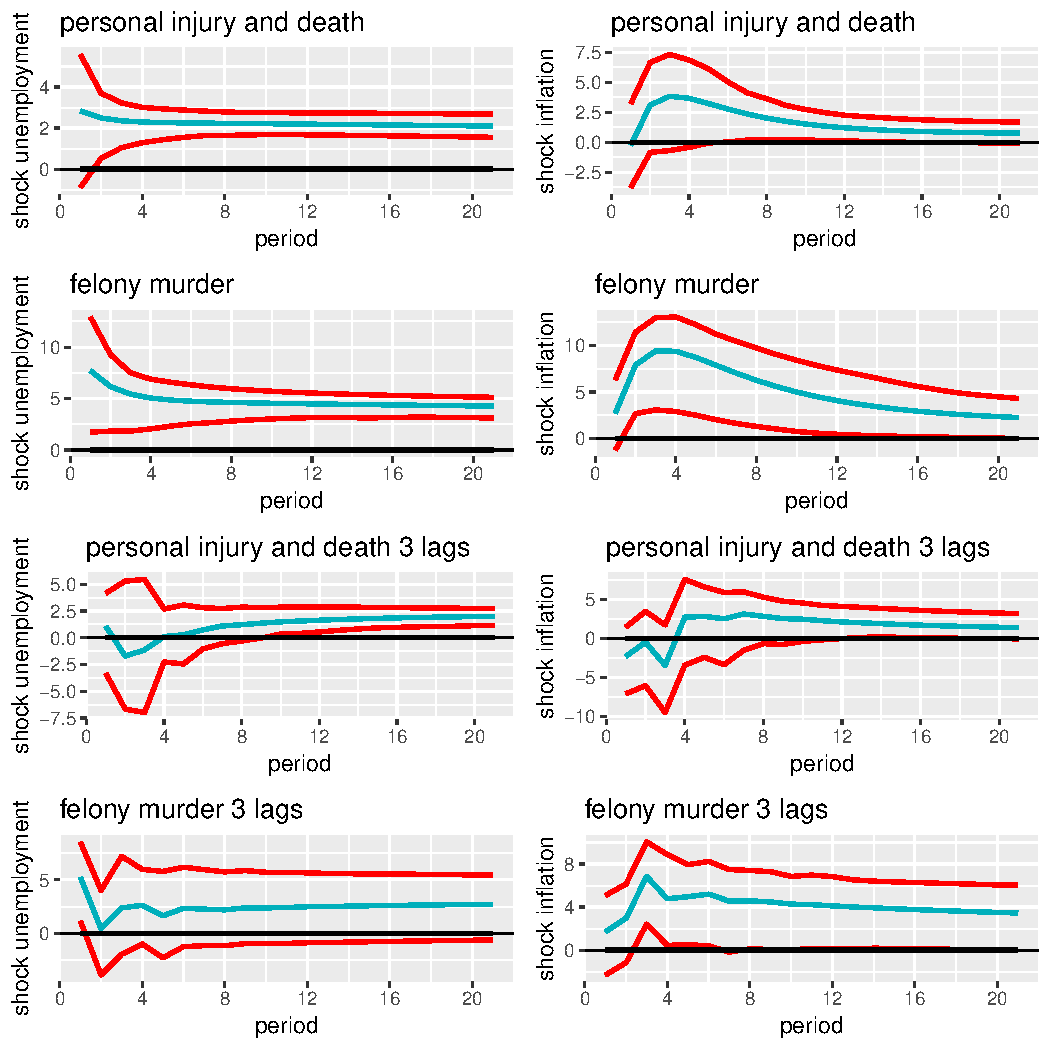
\includegraphics[width=15cm]{graph_irf2}
\label{fig:graph_irf2}
\end{figure}



For personal injury and death and felony murder variables there is serial correlation in the residuals, this is indication that there is more information that can be used if we apply more lags.
As personal injury and death and felony murder are the variables that most respondent to unemployment and inflation  and given that both of them have still serial correlation on the residuals we apply VAR with more lags in these variables. 
A possible reason for felony murder to be relatively more affected is that it has an economic motivation, but rape or homicide e.g. do not have economic motivation. 
The crime of personal injury and death do not necessarily have an economic motivation. An example of this case is a personal motivation to attack someone but without intention to kill the person, the victim is not killed on the spot, but dies some days later.





\begin{table}[H]
\centering 
\caption{VAR results more lags }
\label{tab:VAR_results3}
\begin{tabular}{l l l l  l }\hline\hline 
   & \multicolumn{3  }{c   } {Explained Variables  } \\
Regressors & \textbf{Personal Injury }  & \textbf{Felony Murder }  & \textbf{Felony Murder } \\ 
            & \textbf{and Death 3 lags}  & \textbf{ 3 lags}  & \textbf{ 5 lags}  \\ [4mm] \hline 
$u_{t-1}$ & -7.891 &  -3.043 &   -2.68  \\
$\pi_{t-1}$ & -5.999 &  1274   &  1087 \\
$v_{t-1}$ & 0.2054** &  0.218**    & 0.161*  \\ [4mm]

$u_{t-2}$ & 3.854  &  5.181 &  5.421  \\
$\pi_{t-2}$ & -1379 &  1794  & 2009  \\
$v_{t-2}$ & 0.227*** & 0.301***     &  0.176**  \\ [4mm]

$u_{t-3}$ & 6.328 &-0.475 &  -12.31  \\
$\pi_{t-3}$ & 3096**  & -1072   & -1215   \\
$v_{t-3}$ & 0.219**  &  0.326***  &  0.243***  \\ [4mm]

$u_{t-4}$ & -  & - &  18.72*   \\
$\pi_{t-4}$ &-  &  -   & 122.5  \\
$v_{t-4}$ & - &  -  &  0.066  \\ [4mm]

$u_{t-5}$ & -  &- &  -8.033   \\
$\pi_{t-5}$ & - &  -   & 435.5   \\
$v_{t-5}$ & - &  -   &  0.215**  \\ [4mm]

Normality  & no &  no  &  no \\
Serial Cor. & no & no  &  no   \\
Granger  $ (u,\pi \rightarrow v  )$ & 0.01033 &  0.07943 & 0.1828 \\
\hline\hline
\multicolumn{4}{l}{\footnotesize *  $p < 0.10$, **  $p < 0.05$, ***  $p < 0.01$}\\
\end{tabular}
\end{table}


Table \ref{tab:VAR_results3} show the VAR models with 3 and 5 lags. For personal injury and death with 3 lags only the third lagged inflation is significant, which is a surprise because with the VAR(1) model inflation was not significant and unemployment was. For felony murder with 3 lags, neither unemployment nor inflation are significant. 
But for both models the Granger causality test show significant p-values for the existence of causality. For felony murder with 5 lags unemployment in the fourth lag is significant although there is no Granger causality indication for this number of lags. 
For all models with more lags there is no serial correlation, although there is still non-normality in the residuals.
The IRF graphs for the 3 lagged models do not show the same pattern as the VAR(1) models.

\subsection{Cointegration and VECM }

Given that the variables are not all I(0) we need to test if there is cointegration. We use Johansen cointegration test for the VAR(3) models of personal injury and death and felony murder. We find that both cointegration tests given $r=2$ there are two cointegration relations. We assume that unemployment is the common trend. 




\begin{table}[H]
\centering 
\caption{cointegration vectors}
\label{tab:cointegration_vectors}
\begin{tabular}{l l l l }\hline\hline 
Variable & $ v_t $  &  $ \pi_t $ &  $u_t$ \\ 
Personal Injury and Death I & 1 & 0   & 4.001506  \\
Personal Injury and Death II & 0 &  1  & 0.000137 \\
Felony Murder I & 1 & 0 & -6.1726 \\
Felony Murder II & 0 & 1 & 0.0000475 \\
\hline\hline
\end{tabular}
\end{table}


Table \ref{tab:cointegration_vectors} shows the cointegration vectors. Note that for personal injury and death the sign of unemployment is positive which go against our hypothesis that increasing unemployment increase violence. 
But the sign of felony murder is negative (line ``Felony Murder I"), which is as expected. The other two lines that relate inflation and unemployment are capturing the Phillips curve relation, and have positive signs as is expected for the Phillips curve. 

The cointegration vector shows the long-run relationship between felony murder, unemployment and inflation. Those results agree with the persistent impact of unemployment found in the IRF graphs, but the results do not agree with personal injury and death variable given that the sign of the adjustment coefficient is positive.


\begin{table}[H]
\centering 
\caption{adjustment coefficients}
\label{tab:adjustment}
\begin{tabular}{l| l l l |l l l  }\hline\hline 
 & (1)&(2) & (3)& (4)&(5) & (6)\\ \hline
 & \multicolumn{3}{c}{Personal Injury and Death} & \multicolumn{3}{c}{ Felony Murder}\\
 & $ \Delta v_t $  &  $ \Delta \pi_t $ &  $\Delta u_t$ & $ \Delta v_t $  &  $ \Delta \pi_t $ &  $\Delta u_t$ \\ 
$\alpha_v$ & -0.758*** & 0.000003 & -0.002283**  &  -0.40916*** & 0.0000068  & 0.0029296** \\
$\alpha_\pi$ & -1173 &  -0.3752***  &1.6367  & 1716.8* & -0.3933***  & 3.50038 \\
\hline\hline
\multicolumn{4}{l}{\footnotesize *  $p < 0.10$, **  $p < 0.05$, ***  $p < 0.01$}\\
\end{tabular}
\end{table}

In Table \ref{tab:adjustment}, column 1 shows the adjustment coefficients for equation of violence for personal injury and death variable, columns 2 shows the same but for inflation. Columns 4 shows the adjustment coefficient for violence equation using felony murder variable. 

Column 1's $\alpha_v$ is significant and negative which means that if personal injury and death is too high, the violence measure will decrease to return to the long-run equilibrium. Column 2 and 6's $\alpha_\pi $ are both negative and significant, they say that in the Phillips curve, inflation adjusts. But given that in columns 3 and 6, $\alpha_\pi$ is not significant, unemployment do not adjust in the Phillips curve relationship. 

The signs of $\alpha_v$ in columns 3 and 6 are significant which is a surprise because our hypothesis is that only the violence measure should move to meet the long run relationship, unemployment and inflation can move to meet each others long-run relationship, but between unemployment and violence, for example, only violence should move. For personal injury and death $\alpha_v$ is negative which means that $u_t$ decreases when there is a positive error in the long-run relationship, this is unexpected. Here unemployment is moving away from violence and violence is following unemployment. For the sign of $\alpha_v$ of felony murder is as expected, when there is a positive error in the cointegration relation, unemployment will move to meet the long-run relationship.
\cite{santos_kassouf2014} found in the adjustment coefficients that violence adjust to deviations 
in the long-run relationship.
\cite{saridakis2004}  did not found cointegrating vector. And he found that economic variables 
have a stronger relationship with his murder variable.  
For the short-run coefficients we found no evidence of unemployment and inflation affecting violence measures, the estimates were all statistically insignificant.






\section{Concluding Remarks}




The objective of this work is to study the relationship of violent crimes and economic variables using VAR/VEC models. We analyze the variables in level and rate of change. The violence measures studied are: i) rape; ii) homicides; iii) vehicle theft; iv) vehicle robbery; v) personal injury and death; vi) felony murder. 

The VAR analysis show that all variables behave as expected the sign of shocks in unemployment and inflation increase violence. But for rape and vehicle theft we do not find statistically significant Granger causality estimates. For homicide, vehicle robbery, personal injury and death, and felony murder there is Granger causality. The IRF shows that the shock of unemployment is positive and persistent in time, it does not diminish with time. Inflation shock increase in the first 3 to 4 months and then slowly decreases. 

For personal injury and death and felony murder we test VAR models with three and five lags given that the speciafication with one lag showed serial correlation in residuals and that with those variables the VAR(1) estimates are the most significant. The estimates show that inflation and unemployment are significant, and there is Granger causality from unemployment and inflation to violence. 

We apply a cointegration test on felony murder and personal injury and death. We find  2 cointegration vectors for both variables. The signs of in the cointegrating vectors for felony murder are as expected, when unemployment increases violence increases. But for personal injury and death the long-run relationship coefficients are not as expected. 

The adjustment coefficients for violence in both variables are significant, that means that when violence too high, it decreases to meet the long-run relationship. The adjustment coefficients of unemployment and inflation are significant, which means that they move to the long-run relation. This indication that the cointegration test is capturing the Phillips curve relation. 

This study found evidence that unemployment specially and inflation have significant impact in violence measures. We show that the motivational effect is more important to explain the relationship than the opportunity effect. We found long-run relationships between unemployment, inflation and violence measures.

Further studies should look to the relationship between inflation, unemployment and crime in states or regions of Brazil, study misdemeanor crimes such as: petty theft, prostitution, public intoxication, simple assault, disorderly conduct, trespass, vandalism, reckless driving, discharging a firearm within city limits, possession of cannabis. To capture long-run relations maybe is best to use data with lower frequencies: annual or quarterly. Further studies could use variables of violence measured by population size, one hundred thousand inhabitants. And given that structural changes occur in society we should analyze regime shifts within the series. 









\begin{footnotesize}
\bibliography{references}
\end{footnotesize}










\end{document}






















